\documentclass[fleqn,usenatbib]{mnras}
%@arxiver{picture-havana-vp.png}

%%%%%%%%%%%%%%%%%%%%%%%%%%%%%%%%%%%%%%
%PACKAGES
%%%%%%%%%%%%%%%%%%%%%%%%%%%%%%%%%%%%%%
\usepackage{newtxtext,newtxmath}
\usepackage[T1]{fontenc}
\usepackage{ae,aecompl}
\usepackage{algorithm}
\usepackage[noend]{algpseudocode}
\usepackage{hyperref}
\usepackage{color}
\usepackage{float}
%\restylefloat{table}
\usepackage{placeins}
\usepackage{graphicx}	% Including figure files
\usepackage{amsmath}	% Advanced maths commands
\usepackage{amssymb}	% Extra maths symbols
\setlength{\parindent}{10pt}
\usepackage{caption}

%%%%%%%%%%%%%%%%%%%%%%%%%%%%%%%%%%%%%%
%MACROS
%%%%%%%%%%%%%%%%%%%%%%%%%%%%%%%%%%%%%%
\newcommand{\sub}[1]{_{\rm #1}}
\renewcommand{\sup}[1]{^{\rm #1}}
\newcommand{\vinf}{v_\infty}
\newcommand{\vimp}{v\sub{imp}}
\newcommand{\vearth}{v\sub{\oplus}}
\newcommand{\vesc}{v\sub{esc}}
\renewcommand{\deg}{^\circ}
\newcommand{\beq}{\begin{equation}}
\newcommand{\eeq}{\end{equation}}
\newcommand{\vvec}{\vec{v}}
\newcommand{\GoogleEarth}{{\tt Google Earth}}

\renewcommand{\check}[1]{\textcolor{red}{#1}}
\newcommand{\hll}[1]{#1}
\newcommand{\mytitle}{Can we predict the impact conditions of meter-sized meteoroids?}

%%%%%%%%%%%%%%%%%%%%%%%%%%%%%%%%%%%%%%
%FRONT MATTER
%%%%%%%%%%%%%%%%%%%%%%%%%%%%%%%%%%%%%%

%\title[Impact conditions prediction]{Are the impact conditions of meter-sized meteoroids predictable?}

\title[Can we predict Impact conditions]{\mytitle}

\author[Zuluaga et.al]{
Jorge I. Zuluaga$^{1}$\thanks{Corresponding author: jorge.zuluaga@udea.edu.co},
Pablo A. Cuartas-Restrepo$^{1}$,
Jhonatan Ospina$^{2}$ and
Mario Sucerquia$^{1}$
\\
$^{1}$Solar, Earth and Planetary Physics Group - SEAP,  Institute of Physics, University of Antioquia, calle 70 No. 52 - 21, Medell\'in (Colombia)
\\
$^{2}$Sociedad Antioque\~na de Astronom\'ia / CAMO group, Medell\'in (Colombia)
}

\date{Accepted XXX. Received YYY; in original form ZZZ}

\pubyear{}

\begin{document}
\label{firstpage}
\pagerange{\pageref{firstpage}--\pageref{lastpage}}
\maketitle

%%%%%%%%%%%%%%%%%%%%%%%%%%%%%%%%%%%%%%%%%%%%%%%%%%%%%%%%%%%%
%ABSTRACT
%%%%%%%%%%%%%%%%%%%%%%%%%%%%%%%%%%%%%%%%%%%%%%%%%%%%%%%%%%%%
\begin{abstract}
%\check{(No references in the abstract!})
A few meter-sized meteoroids impact the atmosphere of the Earth per year. Most (if not all) of them are undetectable before the impact and hence, predicting where and how they will fall, seems to be impossible. In this letter we show compelling evidence that we can constrain, in advance, the dynamical and geometrical conditions of an impact. For this purpose, we analyze the well-documented case of the Chelyabinsk impact and the more recent and smaller Cuba event, whose conditions we additionally estimate and provide here. After applying the {\em Gravitational Ray Tracing} algorithm (GRT) to theoretically ``predict'' the impact conditions of the aforementioned events, we find that the speed, incoming direction and (marginally) the orbital elements, can be constrained in advance, starting only on one hand, with the geographical location and time of the impact, and on the other hand, with the distribution in configuration space of Near Earth Objects (NEOs). Any improvement in our capability to predict or at least to constrain impact properties of medium-sized and large meteoroids, will help us to be better prepared for its potentially damaging effects.
\end{abstract}

\begin{keywords}
methods: numerical -- meteorites, meteors, meteoroids.
\end{keywords}

%%%%%%%%%%%%%%%%%%%%%%%%%%%%%%%%%%%%%
%INTRODUCTION
%%%%%%%%%%%%%%%%%%%%%%%%%%%%%%%%%%%%%
\section{Introduction}
\label{sec:introduction}

Earth is impacted by hundreds to thousands of centimeter-sized meteoroids each year. Meter-sized objects are much less frequent, with just a few of them falling into the Earth every year \citep{Brown2013}.  Most of these events occur at very high altitudes, so their shock waves never reach the surface. Still, they are  detectable by satellites \citep{Chapman1994, Brown2002} and infrasound detectors (see eg. \citep{Silber2011}).  
In a few cases, however, an impact of a meter-sized object (releasing energies in the range of several to hundreds of ktons) may happen over populated areas, posing a real risk over infrastructure and population \citep{Popova2013, Rumpf2015}. 

In the case of large (several hundreds of meters) and well-knwon Near Earth Object (NEOs) whose impact probabilities are not negligible, we can predict in advance where and how the object could impact our planet \citep{Chapman2004, Chesley2005,Rumpf2015}. This is possible because the impactor have been previously observed and its orbital elements are very well-constrained.


%\check{On the other hand}
furthermore, the detection of meter-sized NEOs is slow and difficult \citep{Boslough2015}. Predicting where and how one of these objects will impact our planet at a given time, seems to be an impossible task. Proof of this are the impacts in Chelyabinsk, Benenitra (Madagascar) and recently that of Cuba, which had not been observed prior to the event.

In two recent works, \citet{Zuluaga2017p,Zuluaga2018} introduced a novel numerical technique, the Gravitational Ray Tracing (GRT), intended (among many potential applications) to  compute the probability that at a given time, certain geographical region of the Earth (or any other planetary body) be impacted by an asteroid.  More recently \citet{Zuluaga2019} applied GRT to study the impact of a small object against the moon, testing the technique for the first time in a different context and with a different aim for which it was originally devised.

In this letter we apply GRT (Section \ref{sec:GRT}) to study retrospectively the impact conditions (Section \ref{sec:conditions}) of the best documented atmospheric explosion, the Chelyabinsk impact (Section \ref{sec:events}), and a recent,  smaller, but still energetic event over Cuba.  Our aim here is to check if the ``predictions'' that GRT could make about the incoming direction, speed and orbital element of the potential impactors at the place and time of those events (Section \ref{sec:tratm}), coincide with the observed conditions of the impacts.  

Since, to the date of writing, no full reconstruction of the Cuba event has been done (combining infrasound, satellite data and images we expect the atmospheric trajectory and orbit will be precisely reconstructed soon), we provide our own estimations of the impact conditions as obtained from public footage using the methods in \citealt{Zuluaga2013} (Section \ref{sec:supplementary}).

%%%%%%%%%%%%%%%%%%%%%%%%%%%%%%%%%%%%%
%IMPACT CONDITIONS
%%%%%%%%%%%%%%%%%%%%%%%%%%%%%%%%%%%%%
\section{Impact conditions}
\label{sec:conditions}

We call ``impact conditions'' to the set of bulk geometrical and dynamical properties of a meteoroid impact.

Meter-sized objects, ie. $\lesssim 50$ m, hardly achieve to impact the surface.  They normally explode at high altitude in the atmosphere \citep{Brown2002}. Detonations happen when the atmospheric density increases and the aerodynamic pressure at the leading edge of the impactor surpass the strength of the material \citep{Hills1998}. Typical heights of the detonation and the consequent fragmentation (which depends on the strength of the meteoroid) are between 70-20 km \citep{Svetsov1995,Collins2005}. Usually, a cascade of breakup of the main body can also occur, spreading the material of the meteor over certain area on the planet surface. 

%Only strength meteoroids made mainly of iron can reach the surface in one piece, those that are made of other materials like rock or ice need to be large enough ($>50$ m) and possess enough energy and velocity ($\sim 10$ Mton, 20 km s$^{-1}$) to reach hitting the ground \citep{Chapman1994}. 

We call the intersection between the geoid and a straight line tangent to the atmospheric trajectory of the meteoroid, the ``projected impact point'', and denote their geodetic coordinates with lon$_{\rm imp}$, lat$_{\rm imp}$.

The point in the sky from which the meteoroid seems to come is known as ``the impact Radiant''. We parameterize the radiant here in terms of the Azimuth ($A_{\rm rad}$) and elevation ($h_{\rm rad}$) of the radiant as observed from the projected impact point.

%Moreover, at that time the object is seen coming from a point in the sky at a given altitude and azimuth or right ascension and declination.

Because of the impact speed $\vimp$ (typically between 14-20 km/s) and the fact that the mass of the impactor is larger than the mass of the atmosphere displaced during its penetration, the trajectory of the bolide can be assumed nearly rectilinear until it reaches the upper  troposphere.  Therefore a precise determination of the \textit{projected impact point} and the \textit{radiant} are key to estimate the heliocentric orbital elements, $q$, $e$, $i$, $\Omega$ and $\omega$ (with $q$ the perihelion distance, $e$ the eccentricity, $i$ the orbital inclination, $\Omega$ the longitude of ascending node and $\omega$ the argument of perihelion) of the impactor before its energetic interaction with the Earth's atmosphere. 

%The neighborhood of the Earth is populated by a high amount of NEOs, such orbital elements and physical properties (colour, albedo and size distribution) suggest a classification by families \citep{fu2005, morbidelli2002}. It is very common that objects impacting the Earth came from one of those well defined families.

%%%%%%%%%%%%%%%%%%%%%%%%%%%%%%%%%%%%%
%EVENTS
%%%%%%%%%%%%%%%%%%%%%%%%%%%%%%%%%%%%%
\section{Studied events}
\label{sec:events}

%Many meteor events occur during the year. However not all of them occur close to populated areas.  

%In the last century only a few super bolides have happened over populated areas and been  witnessed by thousands to millions of casual observers. 
%There is very little evidence of human fatalities caused by the impact of a meteoroid. There are only a few cases of damage to objects such as automobiles, as in the case of Peekskill in 1992 \citep{Chapman1994}. 
In recent years, and especially due to the expansion and densification of urban areas and the availability of cheap and pervasive electronic cameras, there have been two major impact events with a large number of witnesses and footage records: the Chelyabinsk event (February 15, 2013) and the recent Cuba event (February 1, 2019). Other relatively large events, such as one in Madagascar (July 27, 2018), had also thousands of witnessed but much less available imagery and data.

Multiple sources of information, including public footage, satellite imagery and data, and records from infrasound networks, has allowed us to determine with incredible detail (at least in the case of Chelyabinsk impact) the impact conditions of these events. 

To the date of writing, no full reconstruction of the Cuba event, combining all the above sources of information, has been still published.  In Section \ref{sec:supplementary}, we provide our own estimations of the impact conditions of the Cuba event, as obtained from public footage and using the methods in \citealt{Zuluaga2013}.

In Table \ref{tab:events} we show the impact conditions of the Chelyabinsk and Cuba events, as obtained from the available literature \citep{Zuluaga2013,Popova2013,Borovivcka2013} and from our own estimations (Section \ref{sec:supplementary}). 

%TTTTTTTTTTTTTTTTTTTTTTTTTTTTTTTTTTTTTTTTTTTTTTTT
%EVENTS
\begin{table}
\centering
\begin{tabular}{lll}
\hline\hline
Property & Chelyabinsk (2013) & Cuba (2019)\\
\hline
\multicolumn{3}{c}{Atmospheric Trajectory}\\
\hline
                &  Ref. 1 & This work \\
Date            & 2013/02/15 & 2018/02/01 \\
Time (UTC)      & 03:20:20 & 18:17:10 \\
lon$_{\rm imp}$ (deg)       & +59.8703* & -83.7822 \\
lat$_{\rm imp}$ (deg)       & +55.0958* & +22.8024 \\
$A_{\rm rad}$ (deg)         & 103.5 & 179 \\
$h_{\rm rad}$ (deg)         & 18.55 & 33.0 \\
$\vimp$ (km/s)  & 19.03 & 18.00 \\
\hline
\multicolumn{3}{c}{Heliocentric Orbit}\\
\hline
                & Ref. 1 & This work \\
$a$ (AU)        & 1.72 & 1.32 \\
$e$             & 0.571 & 0.44 \\
$q$ (AU)        & 0.738 & 0.75 \\
$i$ (deg)       & 4.98 & 11.68 \\
$\Omega$ (deg)  & 326.459 & 132.55 \\
$\omega$ (deg)  & 107.67 & 283.8 \\
$P$ (years)     & 2.33 & 1.52 \\ 
$T_p$**           & 2.72 & 2.78 \\ 
\hline\hline
\multicolumn{3}{l}{\footnotesize Ref. 1 \citealt{Borovivcka2013}}\\
\multicolumn{3}{l}{*Ref. 2 \citealt{Zuluaga2013}}\\
\multicolumn{3}{l}{
**Tisserand parameter, $T_p=1/a+2\cos i\sqrt{a(1-e^2)}$ 
}
\end{tabular}
\caption{Impact conditions of the impact events studied in this work.\label{tab:events}}
\end{table}
%TTTTTTTTTTTTTTTTTTTTTTTTTTTTTTTTTTTTTTTTTTTTTTTT

%FFFFFFFFFFFFFFFFFFFFFFFFFF
\begin{figure*}
  \centering
  \vspace{0.2cm}
   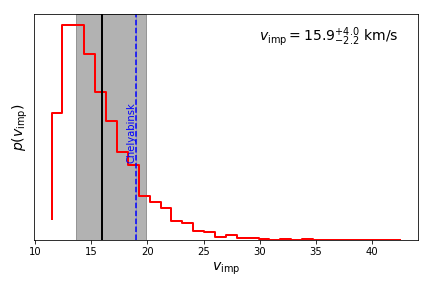
\includegraphics[scale=0.38]{vimp-ppd-Chelyabinsk.png}\hspace{0.1em}%
   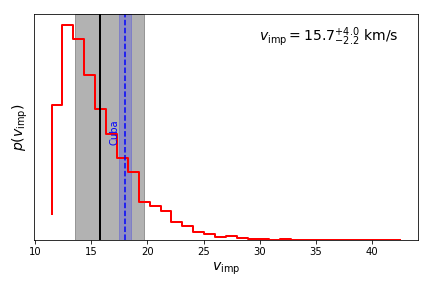
\includegraphics[scale=0.38]{vimp-ppd-Cuba.png}
   \\
   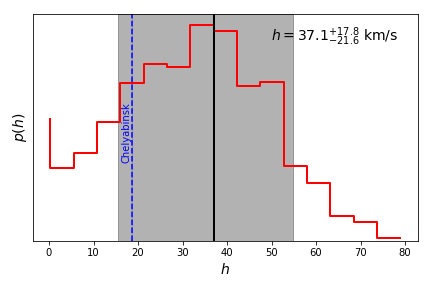
\includegraphics[scale=0.38]{h-ppd-Chelyabinsk.png}\hspace{0.1em}%
   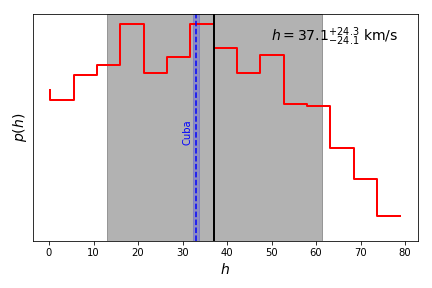
\includegraphics[scale=0.38]{h-ppd-Cuba.png}
   \\
   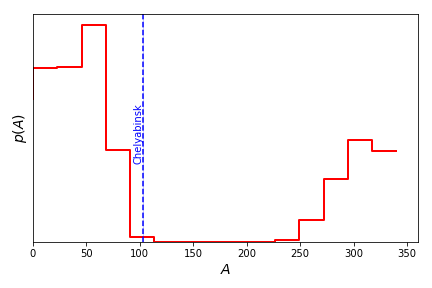
\includegraphics[scale=0.38]{Az-ppd-Chelyabinsk.png}\hspace{0.1em}%
   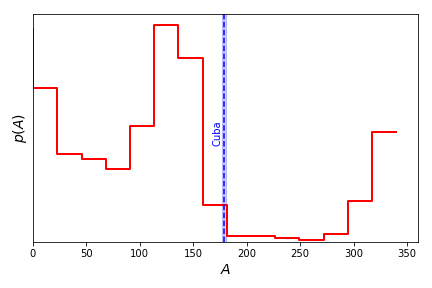
\includegraphics[scale=0.38]{Az-ppd-Cuba.png}
  \caption{Marginal probability distributions of impact velocity, high and azimuth for Chelyabinsk (left panels) and Cuba (right panels) events.}
\label{fig:marginal}
\end{figure*}
%FFFFFFFFFFFFFFFFFFFFFFFFFF

%%%%%%%%%%%%%%%%%%%%%%%%%%%%%%%%%%%%%
%GRT
%%%%%%%%%%%%%%%%%%%%%%%%%%%%%%%%%%%%%
\section{Gravitational Ray Tracing}
\label{sec:GRT}

Are the impact of meter-sized meteoroids and their conditions predictable?  As stated above, the small size of the objects involved on the events studied here, mostly prevent their early  detection, rendering very improbable, if not impossible to anticipate their place and conditions of arrival.  

%One possible way to know the conditions of a given impact will be to integrate many of the NEOs and see which of them could impact the Earth or the Moon in the future. This method, however, is inefficient.

\citet{Zuluaga2017p,Zuluaga2018} (hereafter ZS2018) developed 
and tested a backward integration technique intended to compute the statistical properties of impact conditions. The technique was inspired in the ray tracing algorithms used in the film and game industries to render photorealistic images (see eg. \citealt{Comninos2010} and references there in).  

In GRT, we randomly generate N different impact velocities (regularly spaced between the Earth's escape velocity and that of the Solar System as measured at the orbit of our planet) and M random incoming directions, following a blue-noise distribution to avoid aliasing sampling effects (see Section 2.1 in ZS2018).  Starting at a given impact site and a desired date and time, we integrate backwards the trajectory of this $N\times M$ test particles in the Solar System gravitational field.  The integration stops when test particles reach an asymptotic heliocentric orbit. 

The probability that a test particle, having impact conditions $(A,z,\vimp)$, correspond to a real meteoroid, is given by the so-called {\it ray probability}:

\begin{eqnarray}
\label{eq:ImpactProbabilityDiscreteFlux}
P(A,z,\vimp;t)&\propto& f(\theta\sub{apex},\lambda\sub{apex}) R(q,e,i,\Omega,\omega).
\end{eqnarray}

Here $R(q,e,i,\Omega,\omega)$ is the number density of NEOs in the orbital elements space. In order to correct for the ``defocusing''  effect that the relative motion of the Earth has with respect to the NEOs population (see Section 2.5 in ZS2018), we introduce a flux correcting factor $f$:

\begin{eqnarray}
f(u=\cos[90-\theta\sub{apex}];a,b)&=&
\left\{
\begin{array}{ll}
u^a & -1\leq u < 0; \\
u^b & 0\leq u \leq 1.
\end{array}
\right., 
\label{eq:Flux}
\end{eqnarray}

where $\theta_{\rm apex}$ and $\lambda_{\rm apex}$ are the polar and azimutal angle of the incoming direction with respect to the apex (direction of motion of the Earth). $a\approx 1$ and $b\approx 0.5$ are constants that we fit using the frequency as a function of apex angle of bolides in the NASA fireball database \footnote{\url{https://cneos.jpl.nasa.gov/fireballs/}}.

The number density of NEOs around a point $\vec{x}\equiv(q,e,i,\Omega,\omega)$ in configuration space is estimated with:

\begin{eqnarray}
R(\vec x) &=& \sum_k W(||\vec{x}-\vec{x}_k||,h),
\label{eq:SmoothingFunction}
\end{eqnarray}
 
where $||\vec{x}-\vec{x}_k||$ is a generalized ``distance'' and $h$ a scale parameter.  $W(||\vec{x}-\vec{x}_k||,h)$ is called the {\it smoothing kernel}, and it is intended to soft the transition from a discrete to a continuous regime (see Eq. 7 in ZS2018). 

Distances in configuration space $||\vec{x}-\vec{x}_k||$ are computed using the \citet{Zappala1990} metric with the parametrization introduced by \citet{Rozek2011}:

\hll{
\beq
\label{eq:Z-metric}
\begin{array}{lll}
(D_Z/n_m a_m)^2 & = &
\frac{5}{4} (a-a_m)^2/a_m^2 + 
2 (e - e_k)^2 + \\ 
&  & + 2 (\sin i - \sin i_k)^2 +\\
&  & + 
10^{-4} (\Omega - \Omega_k)^2 +
10^{-4} (\varpi - \varpi_k)^2
\end{array} 
\eeq
}

with $a_m=(a+a_k)/2$ the average semi-major axis between, $n_m$ the corresponding orbital mean motion and $\varpi=\Omega+\omega$ the longitude of the perihelion.

%FFFFFFFFFFFFFFFFFFFFFFFFFF
\begin{figure*}
\centering
%\vspace{0.2cm}
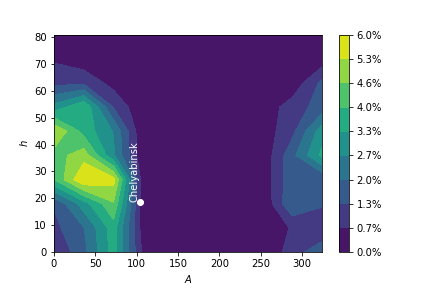
\includegraphics[scale=0.5]{Azh-Chelyabinsk.png}\hspace{1em}%
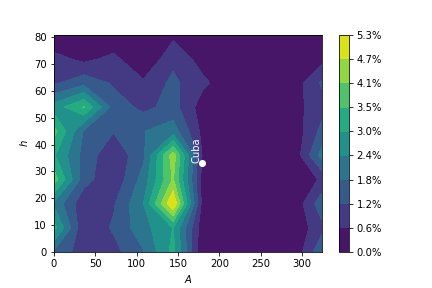
\includegraphics[scale=0.5]{Azh-Cuba.png}
\caption{The estimated radiant for the Chelyabinsk (left panel) and Cuba meteor events (right panel), and the most prone meteoroid radiants in colourmaps according to the GRT technique.}
\label{fig:Azh}
\end{figure*}
%FFFFFFFFFFFFFFFFFFFFFFFFFF

\subsection{Marginal Probabilities}

In ZS2018, we sum-up the ray probabilities at a given geographical location, to compute the (relative) probability that an object impact that location instead of another one.  This allows us to create maps of impact risk.  

But ray probabilities can be used in different ways. Thus, for instance, we can estimate the probability distribution of impact speed, ie.  $p(\vimp)\Delta \vimp$, if we sum-up the ray probabilities having impact speeds in the interval $\vimp, \vimp+d\vimp$:

$$
p(\vimp)d\vimp\propto \sum_{v_{\rm imp,i}\in [\vimp,\vimp+d\vimp]} P(A_i,h_i,v\sub{imp,i};t),
$$

we call this the \textit{marginal probability distribution} of $\vimp$. The same rationale can be applied for computing the marginal probability distribution of any impact condition (radiant elevation, radiant azimuth, asymptotic orbit semi-major axis, etc.). 

In Figure \ref{fig:marginal} we show the marginal probability distributions for several quantities of interest, as computed GRT at the location and time of the Chelyabinsk and Cuba event.  

A similar approach can be generalized to compute two-dimensional marginal probability distributions.  Thus, for instance, the probability that the radiant elevation and Azimuth be in the rectange ${\cal R}:[h_{\rm rad},h_{\rm rad}+dh_{\rm rad}], [A_{\rm rad},A_{\rm rad}+dA_{\rm rad}]$ will given by:

$$
p(A_{\rm rad},h_{\rm rad})dA_{\rm rad}dh_{\rm rad}\propto \sum_{h_{\rm rad,i},A_{\rm rad,i}\in {\cal R}} P(A_i,h_i,v\sub{imp,i};t),
$$

%%%%%%%%%%%%%%%%%%%%%%%%%%%%%%%%%%%%%
%RESULTS
%%%%%%%%%%%%%%%%%%%%%%%%%%%%%%%%%%%%%
\section{Results}
\label{sec:tratm}

As we can notice in Figure \ref{fig:marginal}, the observed impact conditions (speed and incoming directions), for both the Chelyabinsk and Cuba events, are within the statistical errors of the theoretical expectations obtained with GRT. 

The case of the predicted azimuth is especially interesting.  Although the observed value of this quantity in both events, have low marginal probability, GRT predicts the general direction in the sky from which the impactors arrived.  

In the case of Chelyabinks, the GRT predicts a north-east radiant.  In the real world, the object appeared coming from the east.

More interesting is the case of the Cuban meteoroid.  The early records of the American Meteor Society, AMS\footnote{\url{https://fireball.amsmeteors.org/members/imo_view/event/2019/513}} suggested a southbound incoming direction.  The same direction was also suggested by one of the only videos of the event taken from a beach in Florida (see Supplementary Material).  This direction, however, contradicted the GRT expectations of a northbound meteor (lower row in Figure \ref{fig:marginal}) has a larger probability.  This confuse our initial attempts to estimate the trajectory from the available footage.  In the days after the event, new footage and satellite data, confirmed the fact that the meteor actually arrived from the south, as the GRT predicted.

To better understand the level of agreement between the GRT predictions and the observed impact conditions of these events, we plot in Figure \ref{fig:Azh} the joint marginal probability distribution of azimuth and elevation.  

The color maps reveal details that are missing in the independent marginal  probability distributions of azimuth and elevation.  At the date, time and location of the Chelyabinsk event a spot around $A\sim 50^\circ$ and $h\sim 25^\circ$ has the largest probability.  The actual meteor arrived not too far from there.  In the Cuban case, two spots at an azimuth $A\sim 150^\circ$, concentrate most of the expected incoming directions: one at a large elevation $h\sim 30^\circ$ and a second one (and more probable) at low elevation $h\sim 20^\circ$.  The actual event happened close to the first spot.

The elements of the heliocentric orbit of the impactor, shows also interesting coincidences with those predicted by GRT.  In Figure \ref{fig:orbital} we show joint marginal probability distribution for pairs of classical elements. For both events, the orbital elements of the impactor can be well-constrained by the theoretical preditions of GRT. 

%FFFFFFFFFFFFFFFFFFFFFFFFFF
%FIGURE 3
%FFFFFFFFFFFFFFFFFFFFFFFFFF
\begin{figure*}  
  \centering
  \vspace{0.2cm}
   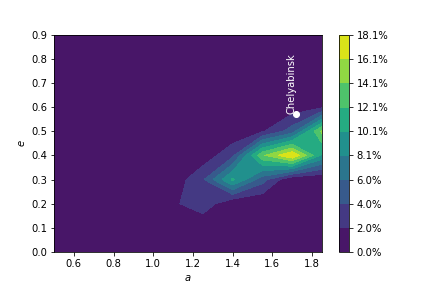
\includegraphics[scale=0.38]{ae-Chelyabinsk.png}\hspace{-0.1em}%
   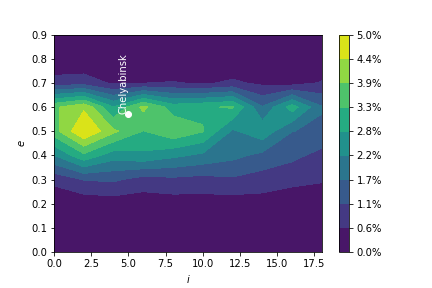
\includegraphics[scale=0.38]{ie-Chelyabinsk.png}\hspace{-0.1em}%
   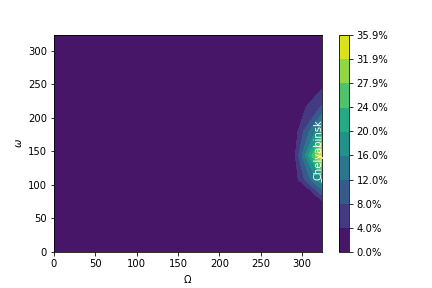
\includegraphics[scale=0.38]{Wo-Chelyabinsk.png}
   \\
   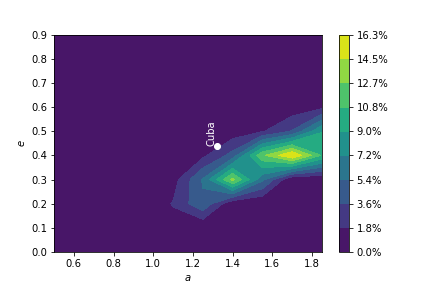
\includegraphics[scale=0.38]{ae-Cuba.png}\hspace{-0.1em}%
   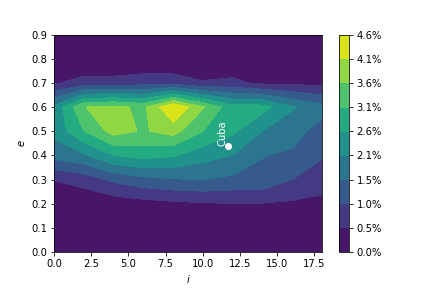
\includegraphics[scale=0.38]{ie-Cuba.png}\hspace{-0.1em}%
   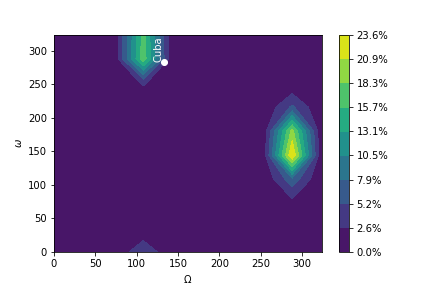
\includegraphics[scale=0.38]{Wo-Cuba.png}\hspace{-0.1em}%
\caption{Colourmaps show the regions in the configuration ($a$, $e$, $i$, $\omega$, $\Omega$) space more prone to impact the Earth at the time and place of Chelyabinsk (uppermost panels) and Cuban meteors (lowermost panels). }
\label{fig:orbital}
\end{figure*}
%FFFFFFFFFFFFFFFFFFFFFFFFFF

Especially noticeable are the case of inclination.  For Chelyabinsk, GRT predicts a low inclination impactor with a moderate $e\sim0.4-0.6$ eccentricity.  The actual impactor has a $i\approx 5^\circ, e\approx 0.6$ orbit.   For Cuba, GRT anticipated relatively eccentric impactor $e\sim 0.6$ coming from a more inclined orbit $i\sim 8^\circ$.  The actual body had $i\approx 11^\circ, e\approx 0.4$.  

The longitude of the ascending node $\Omega$ seems to be easy to predict.  It will mostly depend on the ecliptic longitude of the Earth at the time of impact. However the argument of the perihelion $\omega$, namely the orientation of the axes of the ellipse in the orbital plane, is not as trivial to predict.  Still, GRT anticipates reasonably well the value of $\omega$ for both events.

Interestingly, the orbit of the Chelyabinsk and Cuba impactors are similar.  They have comparable eccentricities and inclinations.  This may be explained by the fact that both impact happened in the same month and hence at a similar orbital position with respect to the NEOs distribution.

\section{Discussion}
\label{sec:discussion}

We started this letter by formulating a strong question: {\it \mytitle?}.  After examining the evidence presented here we propose a bold answer: {\it yes, we can predict them}.  

But this answer should not surprise us.  As the GRT method intrinsically assumes, the NEOs population acts like a gravitational ``source of light'' that instead of photons sends particles towards the Earth.  Predicting the incoming impact direction is a simple consequence of knowing the properties of such body source.

Is GRT perfect and their predictions entirely reliable?. Probably not in its present version. As the differences between the predicted impact conditions and the observed ones seems to reveal, the method can be still improved. We should recall that this and the results in \citet{Zuluaga2019}, are the first attempts to apply the method besides the test bench described in ZS2018.  Better results could be obtained once we have a better knowledge of the NEOs distribution when new and more powerful surveys see their first light \citep{Marshall2017}. The method should also be improved from a theoretical point of view, but it is hard for a single group of authors to achieve it.

Being able to constraint impact conditions will not solve all the risks imposed by small undetectable objects.  Still, it can help us to be prepared for future events, especially over populated areas.  With this work, we also want to call the attention of governmental and no governmental institutions about the interest that theoretical research on impact risk assessment may have, and the potential that novel methods like GRT have at finding answer to what were considered unsolvable questions.  We should implement real time programs for real time impact probability calculations, at least on the most populated cities on the world, 

Our results here relied in our estimations of the Cuba meteor conditions.  Although probably better values of those conditions, obtained after combining all the available information about the event, will be published in the near future, we are confident that the conclusions of this letter will not be substantially modified.
 
%Every effort we do to understand these events and/or to anticipate them, it is very important for our own survival. 

%with the aim of creating a early-alarm impact program and so, with a hand of carefully observations and track of the PHAs (Potentially Hazardous Asteroids), prevent future disasters caused by meteors.  

%interested in public security. It is well-known that several NEOs have a non-zero probability of collision with the Earth within the next 80 years. At least 261 objects between 30 - 300 m are considered potentially dangerous. The distribution of these possible impacts on the surface of the Earth and which countries would have a higher risk is still unknown \citep{Rumpf2015}. 


%Just a couple of weeks after the serendipitous discovery of a meteoroid impact against the Moon \citep{Zuluaga2019}, a new meteorite case were witnessed in the western Cuba town of Vi\~nales. While it is true that the Earth's surface is constantly bombarded by asteroids and  meteoroids, it is rarely possible to have objective and sufficient information to reconstruct the trajectory of the impactor object towards its origins in the interplanetary space. Fortunately, with the advent of the \textit{digital era}, events like Chelyabinsk and Cuba meteor could have been recorded by hundreds of amateur and public video vigilance systems, enabling the full reconstruction of the path of the impactor body.

%In spite of the fact that orbital reconstruction of meteoroids paths towards their original families are currently very common, a new step-forward in the predictability of impact against some particular location on the surface of the Earth and at some particular time have been recently performed by \citep{Zuluaga2018}. GRT Allows both tasks: find the more prone orbital elements of the meteoroid, allowing the identification of the progenitor family, and give an estimation of the RIP on a place at some time, predicting even, the most prone radiant in the sky (See \ref{fig:Azh}).   

%By the application of the GRT to the Cuban and Chelyabinsk meteor events, we obtained a set of orbital osculating elements for each case. On one hand, the similarities between these values suggest a common source, the Apollo asteroids, such orbits cross the orbit of the Earth. However, the belonging of the Cuba meteor to the Apollo family is not completely guaranteed because we estimated a difference of about  $\Delta \omega \sim 100^{\circ}$  between their orbital orientations. On the other hand, a cursory analysis on the composition of the Cuba meteor suggests the presence of small nodules of "troilita", a mineral that was also detected in the fragments recovered from the Chelyabinsk event. 

%In addition, these calculations coincides with the more prone regions in the configuration space of osculating orbital elements calculated with GRT such its collisions probability are high. In other words, GRT have had success to pinpoint the radiants and the intervals of orbital elements potentially hazardous in a specific spatio-temporal coordinate on Earth.

%%%%%%%%%%%%%%%%%%%%%%%%%%%%%%%%%%%%%
%ACKNOWLEDGMENTS
%%%%%%%%%%%%%%%%%%%%%%%%%%%%%%%%%%%%%
\section*{Acknowledgements}

We have used NASA's ADS Bibliographic Services. Most of the computations that made possible this work were performed with NASA NAIF SPICE Software (\citealt{Acton1996} and Jon D. Giorgini), {\tt Python 2.7} and their related tools and libraries, {\tt iPython} \citep{Perez2007}, {\tt Matplotlib} \citep{Hunter2007}, {\tt scipy} and {\tt numpy} \citep{Van2011}. We thank all the people in Cube who shared their videos and footage on the internet, for allowing us to reconstruct the Cuba meteor impact conditions.  We are especially grateful to Rachel Cook who share its incredible video of the meteor from the Havana Harbor which was instrumental for the successful reconstruction of the trajectory.  Karls Pe\~na and Rafael Colon of the Dominican Astronomical Society Astrodom (the Dominican Republic) help us with the non-trivial task of finding information in Cuba about the meteor and the observation places, thanks to them for their effort. 

%%%%%%%%%%%%%%%%%%%%%%%%%%%%%%%%%%%%%
%REFERENCES
%%%%%%%%%%%%%%%%%%%%%%%%%%%%%%%%%%%%%
\begin{thebibliography}{}
\makeatletter
\relax
\def\mn@urlcharsother{\let\do\@makeother \do\$\do\&\do\#\do\^\do\_\do\%\do\~}
\def\mn@doi{\begingroup\mn@urlcharsother \@ifnextchar [ {\mn@doi@}
  {\mn@doi@[]}}
\def\mn@doi@[#1]#2{\def\@tempa{#1}\ifx\@tempa\@empty \href
  {http://dx.doi.org/#2} {doi:#2}\else \href {http://dx.doi.org/#2} {#1}\fi
  \endgroup}
\def\mn@eprint#1#2{\mn@eprint@#1:#2::\@nil}
\def\mn@eprint@arXiv#1{\href {http://arxiv.org/abs/#1} {{\tt arXiv:#1}}}
\def\mn@eprint@dblp#1{\href {http://dblp.uni-trier.de/rec/bibtex/#1.xml}
  {dblp:#1}}
\def\mn@eprint@#1:#2:#3:#4\@nil{\def\@tempa {#1}\def\@tempb {#2}\def\@tempc
  {#3}\ifx \@tempc \@empty \let \@tempc \@tempb \let \@tempb \@tempa \fi \ifx
  \@tempb \@empty \def\@tempb {arXiv}\fi \@ifundefined
  {mn@eprint@\@tempb}{\@tempb:\@tempc}{\expandafter \expandafter \csname
  mn@eprint@\@tempb\endcsname \expandafter{\@tempc}}}

\bibitem[\protect\citeauthoryear{Acton~Jr}{Acton~Jr}{1996}]{Acton1996}
Acton~Jr C.~H.,  1996, Planetary and Space Science, 44, 65

\bibitem[\protect\citeauthoryear{Borovi{\v{c}}ka, Spurn{\`y}, Brown, Wiegert,
  Kalenda, Clark  \& Shrben{\`y}}{Borovi{\v{c}}ka
  et~al.}{2013}]{Borovivcka2013}
Borovi{\v{c}}ka J.,  Spurn{\`y} P.,  Brown P.,  Wiegert P.,  Kalenda P.,  Clark
  D.,   Shrben{\`y} L.,  2013, Nature, 503, 235

\bibitem[\protect\citeauthoryear{Boslough, Brown  \& Harris}{Boslough
  et~al.}{2015}]{Boslough2015}
Boslough M.,  Brown P.,   Harris A.,  2015, in Aerospace Conference, 2015 IEEE.
  pp 1--12

\bibitem[\protect\citeauthoryear{{Brown}, {Spalding}, {ReVelle}, {Tagliaferri}
  \& {Worden}}{{Brown} et~al.}{2002}]{Brown2002}
{Brown} P.,  {Spalding} R.~E.,  {ReVelle} D.~O.,  {Tagliaferri} E.,   {Worden}
  S.~P.,  2002, \mn@doi [\nat] {10.1038/nature01238}, \href
  {https://ui.adsabs.harvard.edu/\#abs/2002Natur.420..294B} {420, 294}

\bibitem[\protect\citeauthoryear{Brown et~al.,}{Brown et~al.}{2013}]{Brown2013}
Brown P.,  et~al., 2013, Nature, 503, 238

\bibitem[\protect\citeauthoryear{Chapman}{Chapman}{2004}]{Chapman2004}
Chapman C.~R.,  2004, Earth and Planetary Science Letters, 222, 1

\bibitem[\protect\citeauthoryear{Chapman \& Morrison}{Chapman \&
  Morrison}{1994}]{Chapman1994}
Chapman C.~R.,  Morrison D.,  1994, Nature, 367, 33

\bibitem[\protect\citeauthoryear{Chesley}{Chesley}{2005}]{Chesley2005}
Chesley S.~R.,  2005, Proceedings of the International Astronomical Union, 1,
  215

\bibitem[\protect\citeauthoryear{{Collins}, {Melosh}  \& {Marcus}}{{Collins}
  et~al.}{2005}]{Collins2005}
{Collins} G.~S.,  {Melosh} H.~J.,   {Marcus} R.~A.,  2005, \mn@doi [Meteoritics
  and Planetary Science] {10.1111/j.1945-5100.2005.tb00157.x}, \href
  {http://adsabs.harvard.edu/abs/2005M%26PS...40..817C} {40, 817}

\bibitem[\protect\citeauthoryear{Comninos}{Comninos}{2010}]{Comninos2010}
Comninos P.,  2010, Mathematical and computer programming techniques for
  computer graphics.
Springer Science \& Business Media

\bibitem[\protect\citeauthoryear{Hills \& Goda}{Hills \&
  Goda}{1998}]{Hills1998}
Hills J.~G.,  Goda M.~P.,  1998, Planetary and space science, 46, 219

\bibitem[\protect\citeauthoryear{Hunter et~al.}{Hunter
  et~al.}{2007}]{Hunter2007}
Hunter J.~D.,  et~al., 2007, Computing in science and engineering, 9, 90

\bibitem[\protect\citeauthoryear{Marshall et~al.,}{Marshall
  et~al.}{2017}]{Marshall2017}
Marshall P.,  et~al., 2017, arXiv preprint arXiv:1708.04058

\bibitem[\protect\citeauthoryear{P{\'e}rez \& Granger}{P{\'e}rez \&
  Granger}{2007}]{Perez2007}
P{\'e}rez F.,  Granger B.~E.,  2007, Computing in Science \& Engineering, 9, 21

\bibitem[\protect\citeauthoryear{Popova et~al.,}{Popova
  et~al.}{2013}]{Popova2013}
Popova O.~P.,  et~al., 2013, Science, 342, 1069

\bibitem[\protect\citeauthoryear{Ro{\.z}ek, Breiter  \& Jopek}{Ro{\.z}ek
  et~al.}{2011}]{Rozek2011}
Ro{\.z}ek A.,  Breiter S.,   Jopek T.,  2011, Monthly Notices of the Royal
  Astronomical Society, 412, 987

\bibitem[\protect\citeauthoryear{Rumpf, Lewis  \& Atkinson}{Rumpf
  et~al.}{2015}]{Rumpf2015}
Rumpf C.,  Lewis H.~G.,   Atkinson P.~M.,  2015, Conference Series

\bibitem[\protect\citeauthoryear{Silber, Le~Pichon  \& Brown}{Silber
  et~al.}{2011}]{Silber2011}
Silber E.~A.,  Le~Pichon A.,   Brown P.~G.,  2011, Geophysical Research
  Letters, 38

\bibitem[\protect\citeauthoryear{{Svetsov}, {Nemtchinov}  \&
  {Teterev}}{{Svetsov} et~al.}{1995}]{Svetsov1995}
{Svetsov} V.~V.,  {Nemtchinov} I.~V.,   {Teterev} A.~V.,  1995, \mn@doi
  [\icarus] {10.1006/icar.1995.1116}, \href
  {http://adsabs.harvard.edu/abs/1995Icar..116..131S} {116, 131}

\bibitem[\protect\citeauthoryear{Van Der~Walt, Colbert  \& Varoquaux}{Van
  Der~Walt et~al.}{2011}]{Van2011}
Van Der~Walt S.,  Colbert S.~C.,   Varoquaux G.,  2011, Computing in Science \&
  Engineering, 13, 22

\bibitem[\protect\citeauthoryear{Zappala, Cellino, Farinella  \&
  Knezevic}{Zappala et~al.}{1990}]{Zappala1990}
Zappala V.,  Cellino A.,  Farinella P.,   Knezevic Z.,  1990, The Astronomical
  Journal, 100, 2030

\bibitem[\protect\citeauthoryear{{Zuluaga} \& {Sucerquia}}{{Zuluaga} \&
  {Sucerquia}}{2017}]{Zuluaga2017p}
{Zuluaga} J.~I.,  {Sucerquia} M.,  2017, in Revista Mexicana de Astronomia y
  Astrofisica Conference Series. pp 79--79

\bibitem[\protect\citeauthoryear{{Zuluaga} \& {Sucerquia}}{{Zuluaga} \&
  {Sucerquia}}{2018}]{Zuluaga2018}
{Zuluaga} J.~I.,  {Sucerquia} M.,  2018, \mn@doi [\mnras]
  {10.1093/mnras/sty702}, \href
  {http://adsabs.harvard.edu/abs/2018MNRAS.477.1970Z} {477, 1970}

\bibitem[\protect\citeauthoryear{Zuluaga, Ferrin  \& Geens}{Zuluaga
  et~al.}{2013}]{Zuluaga2013}
Zuluaga J.~I.,  Ferrin I.,   Geens S.,  2013, arXiv preprint arXiv:1303.1796

\bibitem[\protect\citeauthoryear{{Zuluaga}, {Cuartas-Restrepo}, {Ospina},
  {Pichardo}, {Lopez}, {Pena}  \& {Gaviria-Posada}}{{Zuluaga}
  et~al.}{2019}]{Zuluaga2019}
{Zuluaga} J.~I.,  {Cuartas-Restrepo} P.~A.,  {Ospina} J.,  {Pichardo} F.,
  {Lopez} S.~A.,  {Pena} K.,   {Gaviria-Posada} J.~M.,  2019, arXiv e-prints,
  \href {https://ui.adsabs.harvard.edu/\#abs/2019arXiv190109573Z} {p.
  arXiv:1901.09573}

\makeatother
\end{thebibliography}

%%%%%%%%%%%%%%%%%%%%%%%%%%%%%%%%%%%%%
%SUPPLEMENTARY MATERIAL
%%%%%%%%%%%%%%%%%%%%%%%%%%%%%%%%%%%%%
\clearpage
%\onecolumn
\appendix
\label{sec:supplementary}

%%%%%%%%%%%%%%%%%%%%%%%%%%%%%%%%%%%%%
%RETITLE
%%%%%%%%%%%%%%%%%%%%%%%%%%%%%%%%%%%%%

\noindent
{\Large \bf \mytitle}

\noindent
{\it Jorge I. Zuluaga, Pablo A. Cuartas-Restrepo, Jhonatan Ospina and Mario Sucerquia}

\section{Supplementary material}

\subsection{The 2019 Cuba meteor}

The Cuba meteor happened in February 1, 2019 around 18:17 UTC. It was witnessed by thousands in the island and several casual observers in south Florida (USA).  The meteor left a smoke trail and produced a sonic boom that recalled that of Chelyabinsk in 2013.  According to the NASA fireball database \footnote{\url{https://cneos.jpl.nasa.gov/fireballs/}} the meteor detonation released an estimated energy of $1.4$ kt of TNT. 

Here, we reconstruct the trajectory of the meteor in the atmosphere above Cuba and its orbit before the impact,  using for that purpose different footage originally discovered and obtained from {\tt YouTube}, {\tt Instagram} and {\tt Twitter}.  In particular we analyzed three videos taken at different {\it vantage points}, both in Cuba and USA.  Vantage points are separated by between 100 and 400 km ensuring a proper baseline for the reconstruction of the trajectory.

In Table \ref{tab:vantagepoints} we present the position of the vantage points and links to the corresponding footage we use in our reconstruction. 

%TTTTTTTTTTTTTTTTTTTTTTTTTTTTTTTTTTTTTTTTTTTTTTTT
%EVENTS
\begin{table*}
\centering
\begin{tabular}{llllll}
\hline\hline
Location & long. (deg) & lat. (deg) & alt. (m) & Public & Alternative \\\hline
Havana Harbor, Cuba & -82.344343 & 23.13799 & 0 & \url{http://bit.ly/2GwIQqB} & \url{http://bit.ly/2UJ18c2} \\
%
Gull Wing Beach Resrot, FL USA & -81.903714 & 26.419163 & 0 & \url{http://bit.ly/2tgUU7q} & \url{http://bit.ly/2TGGp8A} \\
%
Alameda Pinar del Rio, Cuba & -83.692091 & 22.414536 & 48 & - & \url{http://bit.ly/2thGkMZ} \\\hline
\end{tabular}
\caption{Location of the vantages points where the footage used in this work were taken.  Public links are the original social network material.  Alternative are permanent link to the footage.}
\label{tab:vantagepoints}
\end{table*}
%TTTTTTTTTTTTTTTTTTTTTTTTTTTTTTTTTTTTTTTTTTTTTTTT

\subsubsection{Havana observations}
\label{sec:havana_observations}

Havana observations are based in a Time lapse, recorded on board of a cruiser in the Havana Harbor.  This video is the most complete and precise piece of footage publicly available about the event.  

The video was taken using a {\tt GoPro Hero 5} using the default Time Lapse mode (0.5 seconds between frames). We achieved to recover 11 frames spanning a total of 5 seconds, where the meteor is clearly visible.  

Azimuth and elevation of the meteor were estimated by first identifying several reference buildings on the horizon (see upper panel in Figure \ref{fig:havana_florida}).

%FFFFFFFFFFFFFFFFFFFFFFFFFF
\begin{figure}  
  \centering
  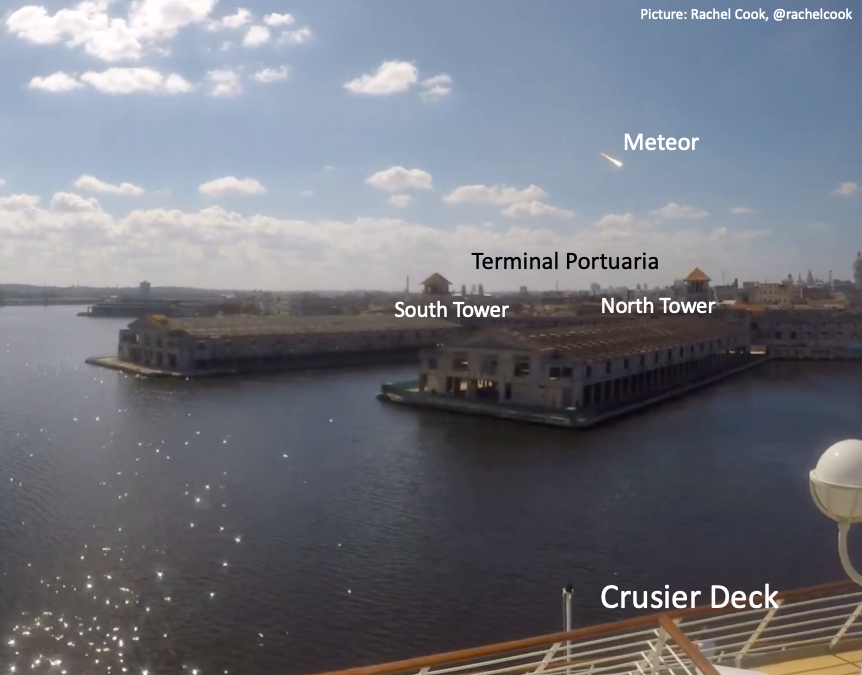
\includegraphics[width=0.50\textwidth]{picture-havana-vp.png}\\
  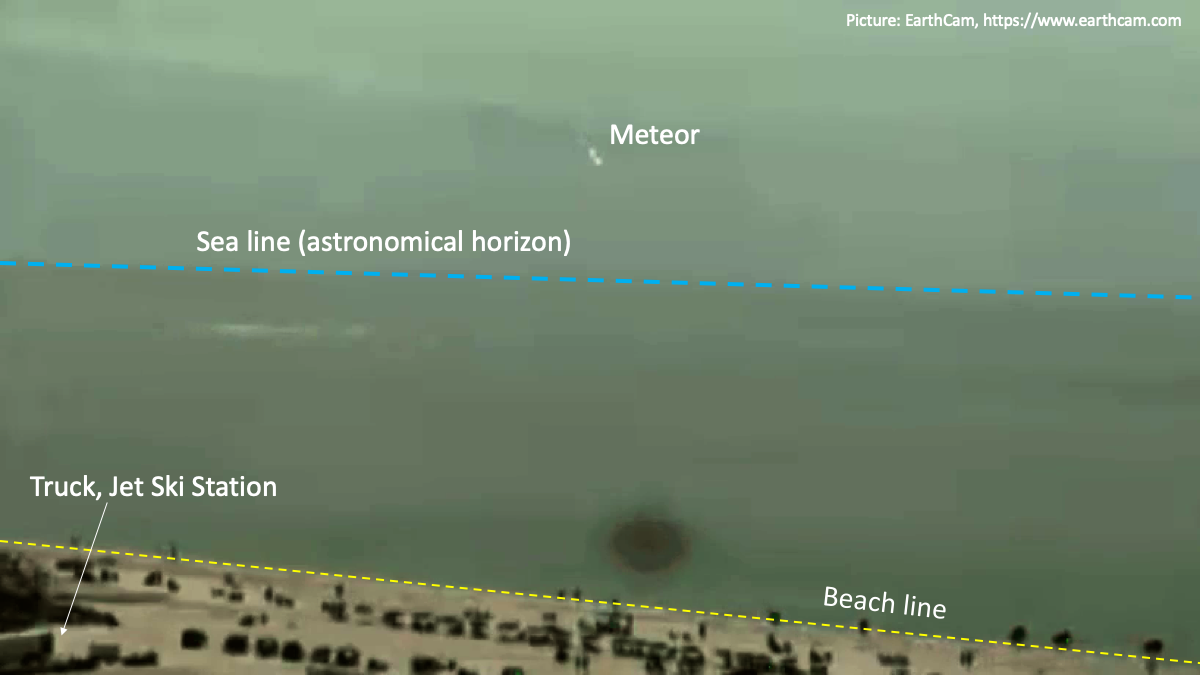
\includegraphics[width=0.50\textwidth]{picture-florida-vp.png}
\caption{Upper panel: a single frame of the video taken in the Havana Harbor showing the reference buildings used in this work to estimate azimuth and elevation of the meteor. Lowe panel: frame of a video taken in the Gull Wing Beach Resort (Floria, USA).\label{fig:havana_florida}}
\end{figure}
%FFFFFFFFFFFFFFFFFFFFFFFFFF

\subsubsection{Florida observations}
\label{sec:florida_observations}

The second footage we use for our reconstruction is a video recorded by a camera of the {\tt Earth Cam} network\footnote{\url{https://www.earthcam.com/}} in the top of the {\it Gull Wing Beach Resort} at Ft. Myers Beach, Florida (USA).  A single frame of the video is shown in Figure \ref{fig:havana_florida}.

Although the quality of the video is poor (as compared with that of the Havana) and the weather near to the Horizons was partially cloudy, we get enough information from the video to estimate the (relative) azimuth and elevation of the meteor.

To obtain the angular scale of the picture, we use as a reference object a truck (or container) apparently used for a jet ski station.  The physical dimensions of the truck or container was obtained from a 3D model of the ``truck'' available in {\tt Google Earth}. Combining the estimated distance between the camera (which is located at the roof of the Resort) and the truck, we calculate the field of view of each pixel in the image.  From that, we estimate the elevation of the meteor in each video frame.

Getting the azimuth of the meteor for this particular image was challenging. No fixed reference object could be identified along the beach.  Therefore, our azimuth measurements were only relative to an arbitrary direction on the horizon.  As we will see below, the precise azimuth of this reference direction was estimated a posteriori using the trajectory fitting procedure (Section \ref{sec:fit}.  

\subsubsection{Pinar del Rio observations}
\label{sec:pinar_observations}

The last footage we used for our reconstruction, was a street video showing the smoke trail left by the meteor. The video, recorded by a casual observer in the city of Pinar del Rio, 173 km to the west of Havana, was particularly well-suited for our purposes, in contrast with most videos recorded in the island, since it was plenty of reference objects able to provide us azimuths and the angular scale of the image. The video was apparently recorded a few minutes after the meteor. The site of the video was plenty identified in \GoogleEarth. 

We stitch together several of the frames in the video, showing the meteor trail and some reference objects, and the result is presented in Figure \ref{fig:pinar}.

%FFFFFFFFFFFFFFFFFFFFFFFFFF
\begin{figure}  
\centering
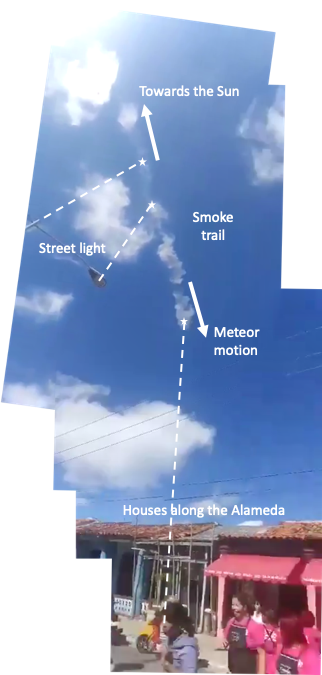
\includegraphics[width=0.3\textwidth]{picture-pinar-vp.png}
\caption{A single frame of the video taken from Pinar del Rio (Cuba), showing the hallmarks used in this work to estimate azimuth and elevation of the meteor.}
\label{fig:pinar}
\end{figure}
%FFFFFFFFFFFFFFFFFFFFFFFFFF

In order to get the elevation and azimuth of several points of the smoke trail, we first need to obtain the angular scale of the picture.  For this purpose we use a lighting street pole located in the opposite side of the street.  According to a source in the island, the height of the lighting street poles in Cuba is Standard. We use this height and the distance of the observer to the pole to gauge the angular scale of the pictures.

The scarce information available in the pictures about the meteor, only allows us to estimate the position of just three points in the smoke trail:

\begin{itemize}
    \item the closest point to the top of a close lighting street pole (see Figure \ref{fig:pinar}). The azimuth of this point was assumed the same as that of the pole (measured using \GoogleEarth).
    \item The point in the smoke trail closer to the lamp in the street pole.  The elevation of this point was obtained after estimating the position of the zenith using the first measurement. A line drawn from the zenith to the lamp allows us to estimate the distance and hence the angle between the lamp and the smoke trail point. The azimuth of this line is the same as the azimuth of the vertical to the lamp as seen from the location of the observer.  The elevation of the lamp was estimated from the distance between the lamp and the observer. 
    \item The lowest point of the trail.  The azimuth of this point was estimated using as references the roof of houses below the trail. \GoogleEarth provided us the azimuth of those houses.  The elevation was estimated using the angular distance between the trail and the ground.
\end{itemize}  

The previous procedure has large uncertainties (several degrees in most of the cases) and it relies mostly on unknown properties (the height of the light pole, the azimuth of the houses, etc.)  Moreover, this procedure give us the observed coordinates of the smoke trail and not of the meteor itself.  Still, in the absence of other more reliable visual recording inside the island, the information provided by this images are priceless.

\bigskip

In Table \ref{tab:measurements} we summarize the observed coordinates (azimuth and elevation) of the meteor as estimated with the aforementioned procedures for the three vantage points.

%TTTTTTTTTTTTTTTTTTTTTTTTTTTTTTTTTTTTTTTTTTTTTTTT
%EVENTS
\begin{table}
\centering
\begin{tabular}{llll}
\hline\hline
Point & Az. (deg) & h (deg) & t (s)\\
%%%%%%%%%%%COPY FROM SCRIPT
\hline\multicolumn{4}{c}{Havana harbor}\\\hline
1 & 223.97 $\pm$ 0.02 & 19.3 $\pm$ 0.08 & 0.00 \\
2 & 225.42 $\pm$ 0.02 & 18.5 $\pm$ 0.08 & 0.50 \\
3 & 226.94 $\pm$ 0.02 & 17.7 $\pm$ 0.08 & 1.00 \\
4 & 228.67 $\pm$ 0.02 & 16.7 $\pm$ 0.08 & 1.50 \\
5 & 230.26 $\pm$ 0.02 & 15.6 $\pm$ 0.08 & 2.00 \\
6 & 232.12 $\pm$ 0.02 & 14.7 $\pm$ 0.08 & 2.50 \\
7 & 233.98 $\pm$ 0.02 & 13.6 $\pm$ 0.08 & 3.00 \\
8 & 235.91 $\pm$ 0.02 & 12.3 $\pm$ 0.5 & 3.50 \\
9 & 237.99 $\pm$ 0.02 & 11.0 $\pm$ 0.5 & 4.00 \\
10 & 240.09 $\pm$ 0.02 & 9.6 $\pm$ 0.5 & 4.50 \\
11 & 242.04 $\pm$ 0.02 & 8.3 $\pm$ 0.5 & 5.00 \\
\hline\multicolumn{4}{c}{GullWing Beach Resort (Florida)}\\\hline
1 & $A_{\rm ref}$+10.1 $\pm$ 0.1 & 2.5 $\pm$ 0.3 & 0.44 \\
2 & $A_{\rm ref}$+10.2 $\pm$ 0.1 & 2.3 $\pm$ 0.3 & 0.50 \\
3 & $A_{\rm ref}$+10.5 $\pm$ 0.1 & 2.0 $\pm$ 0.3 & 0.81 \\
4 & $A_{\rm ref}$+10.8 $\pm$ 0.1 & 1.6 $\pm$ 0.3 & 0.94 \\
5 & $A_{\rm ref}$+11.2 $\pm$ 0.1 & 1.1 $\pm$ 0.3 & 1.94 \\
6 & $A_{\rm ref}$+11.5 $\pm$ 0.1 & 0.8 $\pm$ 0.3 & 2.31 \\
\hline\multicolumn{4}{c}{Pinar del Rio (Cuba)}\\\hline
1 & 287.61 $\pm$ 0.1 & 76.9 $\pm$ 5 & - \\
2 & 308.32 $\pm$ 5 & 68.2 $\pm$ 5 & - \\
3 & 318.07 $\pm$ 5 & 57.8 $\pm$ 5 & - \\
%%%%%%%%%%%COPY FROM SCRIPT
\hline\hline
\multicolumn{4}{l}{\footnotesize*$A_{\rm ref}$ is obtained in the fitting procedure.}\\
\end{tabular}
\caption{Observed trajectory of the meteor in the sky as estimated in this work for three different vantage points.\label{tab:measurements}}
\end{table}
%TTTTTTTTTTTTTTTTTTTTTTTTTTTTTTTTTTTTTTTTTTTTTTTT

\subsection{Trajectory fitting}
\label{sec:fit}

One of the main limitations of working with public or amateur footage is the lack of a proper synchronization among videos. In only two of them (the Havana and Florida videos) we have information about the time of each frame relative to the beginning of the video (last column in Table \ref{tab:measurements}).  No absolute timing was available.  

For solving this inconvenience we developed in \citet{Zuluaga2013} a numerical procedure intended to fit a meteor trajectory, starting only with the measurements of elevations and azimuths. We call it the ``Altazimuth-footprint method''. 

In contrast with the original version of the method, the improved version we use here, involved both, errors in elevation and azimuth to compute the altazimuth-footprint statistics:

\beq
\label{eq:altaz}
\mathcal{A}=\sqrt{
\sum_{j=1}^{n_v}\sum_{i=1}^{n_j} 
\left[
\frac{(A_{ji}-A_{tji})^2}{\Delta A_{ji}^2}+
\frac{(h_{ji}-h_{tji})^2}{\Delta h_{ji}^2}
\right]
}
\eeq

Here, $n_v$ is the number of vantage points, $n_j$ is the number of observations in the $j$th vantage point, $(A_{ji},h_{ji})$ are the horizontal coordinates of the $i$th point in the $j$th vantage point, and $(A_{tji},h_{tji})$ are the azimuth and elevation of the closest point in the theoretical trajectory respectively.

The theoretical trajectory depends on four quantities: the projected impact site location (lon$_{\rm imp}$,lat$_{\rm imp}$) (alt$_{\rm imp}$=0), the radiant azimuth $A_{\rm rad}$ and the radiant elevation $h_{\rm rad}$ as seen from the projected impact site. 

In order to find the best-fit value of those parameters we minimize the statistics ${\cal A}$. Due to the particularities of the Florida footage, we add a fifth parameter to the minimization procedure, namely the reference Azimuth $A_{\rm ref}$ at the Gull Wing Beach vantage point (see Table \ref{tab:measurements}).

The result of the fitting procedure is presented in Table \ref{tab:fit}. Using the best-fit trajectory, we also compute the heliocentric orbit of the meteoroid 1 year before the impact. The resulting classical elements are also shown in this Table.

%TTTTTTTTTTTTTTTTTTTTTTTTTTTTTTTTTTTTTTTTTTTTTTTT
%EVENTS
\begin{table}
\centering
\begin{tabular}{ccc}
\hline\hline
Parameter & Best fit value\\
\hline
\multicolumn{2}{c}{Atmospheric trajectory}\\
\hline
Lon. impact (deg) & -83.78217648 $\pm$ 0.05 \\
Lat. impact (deg) & 22.80238773 $\pm$ 0.05 \\
$A_{\rm rad}$ (deg) & 179 $^{+1}_{-4}$ \\
$h_{\rm rad}$ (deg) & 33 $^{+0.5}_{-1.5}$ \\
$A_{\rm ref}$ (deg) & 192.5 $\pm$ 0.5 \\
$\langle v_{\rm imp}\rangle$ (km/s) & 18.0 $^{+0.3}_{-1.2}$ \\
\hline
\multicolumn{2}{c}{Orbit}\\
\hline
$a$ (AU) & $1.32^{+0.06}_{-0.06}$\\
$q$ (AU) & $0.75^{+0.02}_{-0.02}$\\
$e$ (AU) & $0.44^{+0.02}_{-0.02}$\\
$i$ (AU) & $11.68^{+0.4}_{-0.4}$\\
$\Omega$ (AU) & $132.54^{+0.004}_{-0.003}$\\
$\omega$ (AU) & $283.77^{+3}_{-5}$\\
$P$ (yr) & $1.52^{+0.1}_{-0.1}$\\
$T_p$ (adim.) & $2.78^{+0.02}_{-0.02}$\\
\hline
\end{tabular}
\caption{Best-fit values of the atmospheric trajectory and the asymptotic orbit of the meteoroid for the Cuba impact as estimated in this work.}
\label{tab:fit}
\end{table}
%TTTTTTTTTTTTTTTTTTTTTTTTTTTTTTTTTTTTTTTTTTTTTTTT

A plot with a comparison between the observed meteor trajectory and the best-fit Altazimuthal footprint, is presented in Figure \ref{fig:fit}.

%FFFFFFFFFFFFFFFFFFFFFFFFFF
\begin{figure*}  
  \centering
  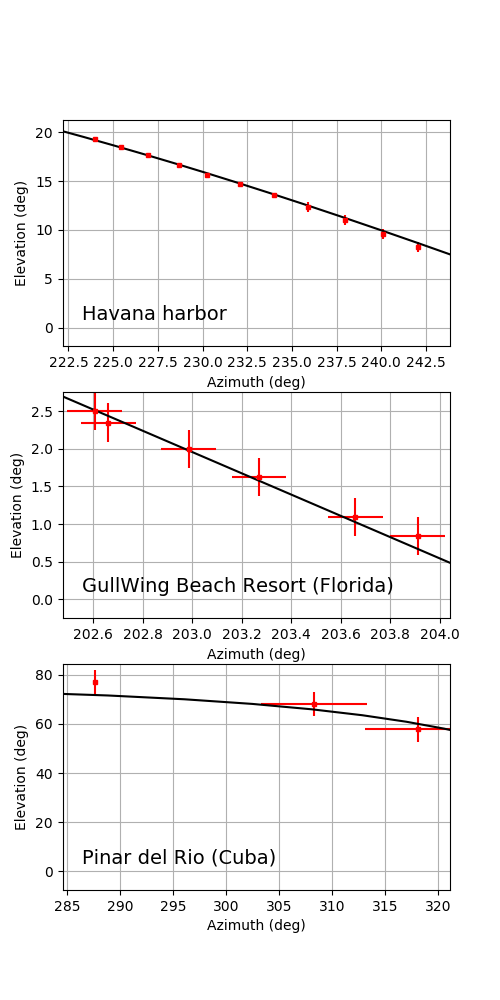
\includegraphics[width=0.4\textwidth]{trajectory-fit.png}
\caption{Expected azimuth and elevation of the theoretical trajectory (continuous line) as observed from the vantage points, and the actual measurements estimated in this work.  In the three cases the horizontal and vertical ranges have been adjusted to the ranges of the available data.\label{fig:fit}}
\end{figure*}
%FFFFFFFFFFFFFFFFFFFFFFFFFF

We found that in order to explain our three visual observations, the object should come almost exactly from the south, traveling in an inclined $h_{\rm rad}=33^\circ$ trajectory towards the north coast of Cuba.  According to the observations in the Havana Harbor the contact point of the object with the atmosphere happened at 76 km above the ocean to the south of San Felipe Cays.  The brightest point in the video corresponds to a point in the trajectory 27 km obove the surface.  

On the other hand, according to our estimations, the smoke trail seen in the Pinar del Rio video, corresponds to a short segment of the trajectory between 26 km and 22.5 km.  The latter point, apparently correspond to the end of the airburst. 

Using our fitted trajectory and the very precise footage taken at the Havana harbor, we can estimate the distance traveled by the meteoroid in the atmosphere as a function of time.  A linear regression of the resulting distances, provide us the average speed of the meteoroid during the airburst.

%FFFFFFFFFFFFFFFFFFFFFFFFFF
\begin{figure*}  
  \centering
  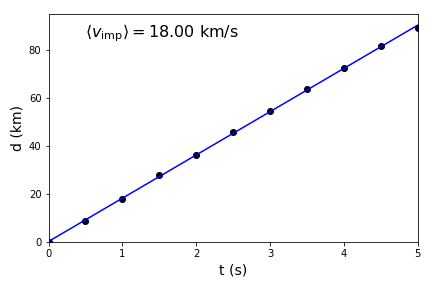
\includegraphics[width=0.45\textwidth]{impact-speed.png}
\label{fig:speed}
\caption{Distance travelled by the meteor using the best-fit trajectory and the Havana Harbor observations (black dots). The blue line corresponds to the linear regression.  The average impact speed $\langle\vimp\rangle$ corresponds to slope of the blue continuous line.}
\end{figure*}
%FFFFFFFFFFFFFFFFFFFFFFFFFF

We see that the speed of the meteoroid was almost constant between 76 km and 26 km height, and started to decrease just after that moment. 

\subsection{Discussion}

The estimated impact conditions, presented here, depends on several assumptions and on the validity of the geometrical procedures used to measure azimuths and elevations over the pictures.  

The most uncertain measurements are those taken at Pinar del Rio.  Since the footage there does not include the visible meteor but the smoke trail, it could happen that the cloud be displaced from the actual meteor trajectory by several degrees. In particular the meteor could happen to the west of the cloud observed position.  In this case the trajectory will be farther away from the Havana Harbor and hence the estimation of the distance traveled by the meteoroid, and hence the impact speed, will also be affected.  

We have played around with the observed coordinates of the Pinar del Rio observations, modifying elevations and azimuths to simulate the effect of the wind.  The errors reported in Table \ref{tab:fit} reflect those uncertainties.

In order to estimate the errors in the orbital elements, we create 1000 test particles having random impact conditions within the intervals defined by the errors in the atmospheric trajectory section of Table \ref{tab:fit}.  The errors reported in the orbital elements are the result of this simulations.  We noticed that even if, for instance the impact speed is as low as 16.8 km/s (the lowest velocity allowed by our footage), the orbital elements are not significantly modified.

\subsection{Reproducibility}

In order to make all our results reproducible, we provide all the input data, simulation results, spreadsheets and crude videos and images, in a public {\tt GitHub} repository: \url{http://github.com/seap-udea/MeteorTrajectories.git}.  The GRT method was implemented in a {\tt C$++$/python} package  also publicly available in the {\tt GitHub} repository \url{http://github.com/seap-udea/GravRay.git} (branch {\tt MoonImpact}).

Any suggestion, observations or corrections will be greatly appreciated.

%%%%%%%%%%%%%%%%%%%%%%%%%%%%%%%%%%%%%
%THE END
%%%%%%%%%%%%%%%%%%%%%%%%%%%%%%%%%%%%%
\bsp
\label{lastpage}
\end{document}
